\documentclass[a4paper,11pt]{article}

\usepackage[utf8]{inputenc}
\title{ARC1 - TP 4}
\author{Léo Noël-Baron \& Thierry Sampaio}
\date{23/10/2015}

\usepackage{a4wide}
\usepackage{textcomp}
\usepackage[utf8]{inputenc}
\usepackage[T1]{fontenc}
\usepackage[francais]{babel}

\usepackage{graphicx}
\usepackage[usenames,dvipsnames]{color}

\usepackage{hyperref} \urlstyle{sf}
\hypersetup{
  colorlinks=true,
  urlcolor=BlueViolet,
  citecolor=BlueViolet,
  linkcolor=BlueViolet,
}
\DeclareUrlCommand\email{\urlstyle{sf}}

\newenvironment{keywords}
  {\description\item[\bsc{Mots-clés}]~$\cdot$~ }
  {\enddescription}
\newenvironment{remarque}
  {\description\item[\bsc{Remarque} ---]\sl}
  {\enddescription}
\renewcommand{\thefootnote}{\arabic{footnote}}

\usepackage{listings}
\lstset{
  language=C,
  basicstyle=\ttfamily,
  keywordstyle=\color{OliveGreen},
  stringstyle=\color{Bittersweet},
  showstringspaces=false,
  commentstyle=\color{Gray},
  numbers=left,
  numberstyle=\ttfamily\color{Gray},
  frame=l,
  columns=fullflexible,
  rulecolor=\color{Gray},
  tabsize=4,
  extendedchars=true,
  literate=
	{É}{{\'E}}1 {è}{{\`e}}1 {à}{{\`a}}1 {È}{{\`E}}1 {À}{{\`A}}1 {ê}{{\^e}}1 {â}{{\^a}}1 {î}{{\^\i}}1 {ô}{{\^o}}1
	{Ê}{{\^E}}1 {Â}{{\^A}}1 {Î}{{\^I}}1 {Ô}{{\^O}}1 {Û}{{\^U}}1 {ë}{{\"e}}1 {ï}{{\"\i}}1 {ü}{{\"u}}1 {Ë}{{\"E}}1
	{Ï}{{\"I}}1 {Ü}{{\"U}}1 {û}{{\^u}}1 {ç}{{\c c}}1 {Ç}{{\c C}}1 {æ}{{\ae}}1 {Æ}{{\AE}}1 {œ}{{\oe}}1 {Œ}{{\OE}}1
	{é}{{\'e}}1,
}
\lstMakeShortInline{|}

\parskip=0.3\baselineskip
\sloppy

\makeatletter
  \let\runtitle\@title
  \let\runauthor\@author
\makeatother

\usepackage{fancyhdr}
\pagestyle{fancy}
\fancyhead{}
\lhead{\runtitle}
\rhead{\runauthor}
\setlength{\headheight}{13.6pt}

\usepackage{amssymb}

\setlength{\parindent}{0em}
\usepackage{array}

\begin{document}

\maketitle

\begin{abstract}
	Ce TP propose l'élaboration d'une Unité Arithmétique et Logique (UAL) simpliste, permettant quatre opérations logiques ainsi que l'addition et la soustraction et traitant des données sur 4 bits. Cette UAL comportera trois opérandes (dont une commande sur 3 bits) et trois sorties (le résultat sur 4 bits et les retenues de l'addition et de la soustraction).
\end{abstract}

\subsection*{Opérations logiques}

\paragraph{ET/ID} On souhaite implémenter les opérations logiques suivantes sur deux opérandes $X$ et $Y$ : $X\wedge Y$, $Y$, $X\wedge \overline{Y}$ et $\overline{Y}$. Pour cela, on réalise tout d'abord un circuit ET/ID qui renvoie $A\wedge B$ ou $B$ selon une commande $\overline{et}$. L'expression formelle correspondant à ce traitement est $S_i=B_i\wedge (A_i\vee\overline{et})$ (pour $i\in[0..3]$), ce qui donne le circuit en Figure \ref{etid}.

\begin{figure}[h]
	\center
	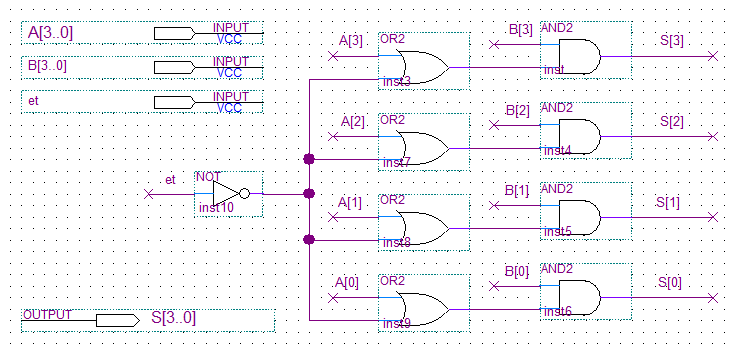
\includegraphics[scale=0.75]{etid.png}
	\caption{Schéma du composant ET/ID}
	\label{etid}
\end{figure}

\paragraph{INVCOND} On conçoit ensuite un inverseur conditionnel au moyen de portes XOR ; l'expression formelle $B_i=A_i\oplus inv$ ($inv$ étant la commande d'inversion) s'implémente comme en Figure \ref{invcond}.

\begin{figure}[h]
	\center
	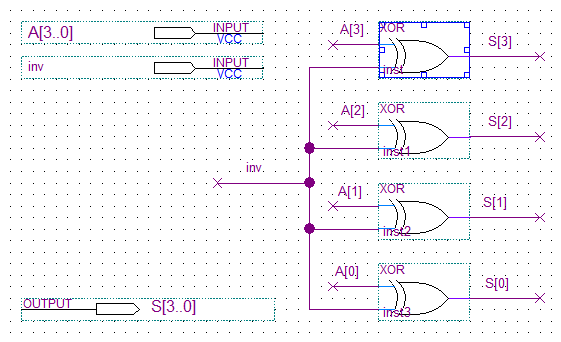
\includegraphics[scale=0.75]{invcond.png}
	\caption{Schéma du composant INVCOND}
	\label{invcond}
\end{figure}

\paragraph{OPLOG} Les deux circuits précédents permettent de construire le circuit d'opérations logiques de l'UAL. En effet, la table des commandes impose pour les deux bits de poids faible
\begin{table}[h]\centering
\begin{tabular}{c|c|c|c|c}
	$L_1L_0$ & 00 & 10 & 01 & 10 \\ \hline
	Opérations & $X\wedge Y$ & $Y$ & $X\wedge \overline{Y}$ & $\overline{Y}$ \\
\end{tabular}\end{table}
ce qui permet directement de commander les circuits ET/ID et INVCOND avec respectivement les signaux $L_1$ et $L_0$ (Figure \ref{oplog}).

\begin{figure}[h]
	\center
	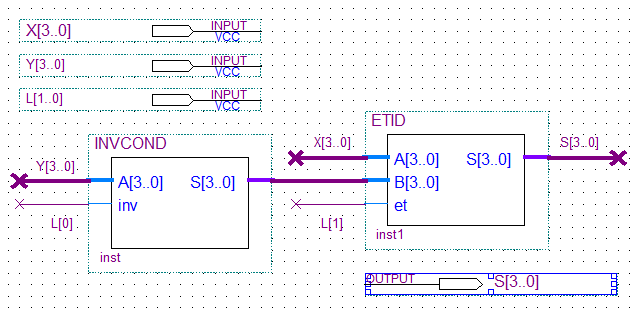
\includegraphics[scale=0.75]{oplog.png}
	\caption{Schéma du composant OPLOG}
	\label{oplog}
\end{figure}


\subsection*{Opérations arithmétiques}

\paragraph{Conception} Le circuit arithmétique de l'UAL prend deux opérandes sur 4 bits $X$ et $Y$, ainsi qu'une commande $AS$ pour choisir l'opération. Il peut être réalisé au moyen des circuits ADD4GROUP et INVCOND ; en effet, la notation en complément à deux se fait en inversant bit à bit une opérande binaire et en lui ajoutant 1. On inverse donc au besoin $Y$ grâce au circuit INVCOND commandé par $AS$, et on redirige le signal dans ADD4GROUP où on réutilise $AS$ en retenue entrante pour obtenir la notation en complément de $Y$.

La retenue sortante et le débordement nécessitent un traitement supplémentaire, différencié selon l'opération. L'addition ne peut donner qu'une retenue sortante, qui est celle de l'additionneur ADD4GROUP. La soustraction donne en retenue sortante l'inverse de celle d'ADD4GROUP, mais peut aussi provoquer un débordement qui est détectable si le résultat est du signe inverse des opérandes. On construit donc le circuit présenté en Figure \ref{addsous}.

\begin{figure}[h]
	\center
	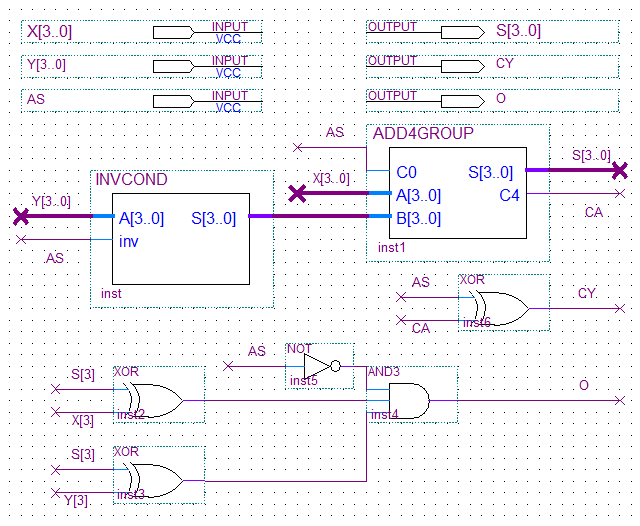
\includegraphics[scale=0.75]{addsous.png}
	\caption{Schéma du composant ADD/SOUS}
	\label{addsous}
\end{figure}

\paragraph{Jeu de test} Pour tester l'addition, on peut effectuer les opérations :
\begin{itemize}
	\item 1001 + 0011 (9 + 3, pas de retenue sortante) et
	\item 0101 + 1101 (5 + 13, retenue sortante).
\end{itemize}
Pour la soustraction :
\begin{itemize}
	\item 1110 - 0011 (14 - 3, pas de retenue mais débordement) ;
	\item 1010 - 0100 (10 - 4, pas de retenue ni de débordement) ;
	\item 0010 - 0101 (2 - 5, retenue mais pas de débordement) et
	\item 0011 - 1101 (3 - 13, débordement).
\end{itemize}


\subsection*{Assemblement de l'UAL}

L'UAL se construit à partir des composants précédemment définis, en dirigeant les opérandes et les signaux de commandes adéquats aux entrées du circuit arithmétique et du circuit logique, puis en sélectionnant le résultat voulu avec un SEL4 ; ceci donne le circuit final présenté en Figure \ref{ual}.

\begin{figure}[h]
	\center
	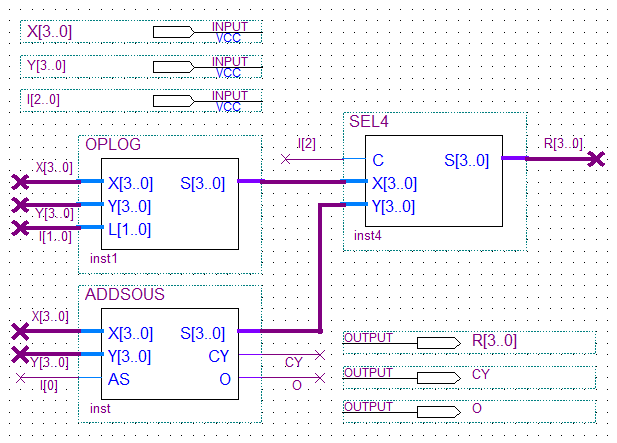
\includegraphics[scale=0.75]{ual.png}
	\caption{Schéma de l'UAL}
	\label{ual}
\end{figure}

\end{document}
